\documentclass[jou,apacite]{apa6}

\usepackage[utf8]{inputenc}
\usepackage[nonumberlist]{glossaries}
\usepackage{makeidx}

\makeglossaries
\loadglsentries{glossary}
\makeindex

\title{A short introduction to artificial intelligence}
\shorttitle{AI intro}

\author{Daniel Schruhl}
\affiliation{ThoughtWorks}

\abstract{A short introduction into the general topic of artificial intelligence. This should help address some aspects of artificial intelligence and define them on a shallow level to give a starting point into this topic.}

\begin{document}
\maketitle    
                        
\section{Motivation}
There are a lot of definitions for \gls{ai}. Most of them are based on a definition of intelligence which in itself is already difficult to define. A simple approach would be to say that humans cognitive functions (e.g. solving complex problems or learning) is considered intelligent. So making programs or machines pursue the way humans might solve problems or learn can be considered as \gls{ai}. These complex problems can be natural language processing, visual perception, motor control, planning or game theory.

\gls{ai} programs are sometimes also considered intelligent because from the outside their outcome appear to be magic. When actually developing the program itself and deep diving into the implementation, it leads to the realization of the often trivial nature of the implementation. This illustrates the possible paradox in \gls{ai}.

\gls{ai} can be used for image recognition, for controlling machines, to play games or to detect fraud. It can be used in nearly any domain and has already found great usage in medicine or commercial scenarios. Using \gls{ai} can give a company a major advantage against competitors. Companies like Netflix have embraced \gls{ai} \cite{Gomez-Uribe2015} and have established a market leading position also backed by \gls{ai}.

\section{Types of \gls{ai}}
Approaches to implement \gls{ai} have resulted into two major paradigms: \textbf{symbolic} and \textbf{sub-symbolic}. Symbolic approaches model a problem space with tokens or symbols that are humanly readable. This problem space is then processed by the \gls{ai} programs. The symbols themselves are therefore manipulated and processed. Because of the symbolic nature the \gls{ai} programs can be completely understood by humans. These programs are often called \gls{expert-system}, \gls{rules-engine}, \gls{knowledge-based-ai} or \gls{knowledge-graph}. They were the first paradigms that found usage in the past and are therefore also called \gls{gofai}. In theory they try to solve modeled problems in the same abstract way humans think and would solve problems.

The sub-symbolic paradigm also consists of symbols but they are not really human interpretable. These symbols represent more abstract components that can accomplish tasks suitable for \gls{ai} related tasks. The whole idea about this paradigm is to build the parts that make human cognitive functions possible on a more low level abstraction. It is highly inspired by biology (neurobiology, genetics, evolution) and psychology. This paradigm has found a lot of usage and popularity in the recent years.

\subsection{\gls{symbolic-ai}}
As stated before symbolic AI solves complex problems by using strategies researchers thought humans would also use. This is done by transforming a problem space into symbols and then applying functions on these symbols. The key here is coming up with an abstract model of the problem space and transforming it into symbols. Because of the nature of this paradigm, expert systems are easier to debug and understand and to control. A big disadvantage is that you need expert domain knowledge in order to solve the problem the way humans would do. Another advantage is though that big data is not needed.

Due to the symbolic nature \textbf{logic} can be used to solve complex problems. Logic consists of \textbf{semantic} and \textbf{syntax}. Syntax defines the representation of logics (symbols). It consists of an alphabet which forms words which in turn form language (\textbf{formulas}). This syntax is then interpreted by semantics. Semantics give meaning and interpretation to syntax and can be used to derive new formulas (\textbf{calculus}). This kind of system is called \textbf{formal system}. For more information about logics and formal systems see \cite{Richardson2006}. 

Formal systems have rules. These rules can be used to infer new rules or answer questions. This is often done by calculus (e.g. resolution calculus). Such a system of \gls{ai} can be built with \gls{prolog}. An example for this would be the task of parsing natural language into semantic compositions. Theoretical computer science can be used to define natural language with grammar. Inside that grammar are symbols like terminal and non-terminal symbols and productions which form rules. These rules can be used to parse natural language into semantic compositions like verbs, nouns or adjectives. These can in turn be used to be processed. This can be done with \textbf{\gls{dcg}} \cite{Wood1990}.

Another important aspect of symbolic AI are \textbf{searches}. In symbolic AI searches are used in finding solutions in a modeled problem space. The solution can be a path leading to a goal or the goal itself. The key aspect here is again modeling the problem space so a search is usable. This could be for example trying to find the perfect schedule for people with limited amount of time. Searches can be simple algorithms (breadth-first, depth-first) or \textbf{informed algorithms} (e.g. $A^*$). Informed algorithms use \textbf{heuristics} that try to estimate the best possible path inside a graph. This should lead to a faster search because some paths can be \textbf{pruned}. The intelligent part here lies in defining the heuristic. An example of an \gls{ai} using pruning and informed search is the Deep Blue chess computer \cite{Campbell2002}.

Another aspect in searches is the \textbf{\gls{csp}}. In a \gls{csp} are \textbf{variables} which have value spaces (\textbf{domains}). Each variable is attached to \textbf{constraints}. These constrains can have multiple arity and define limitations for the domains. 
This way a net of variables and constraints is formed (see figure \ref{fig:cs-net}). The problem of solving the net and narrowing down the domains to a solution is the actual \gls{csp}. To solve these problems there are multiple algorithms (e.g. AC-3). \gls{csp} can be used to solve riddles or puzzles like Sudoku.

\begin{figure}[!htb]
\centering
	\includegraphics[width=.25\textwidth]{csp.pdf}
\caption[Constraint net]{Constraint net with variables $v = \{X,Y,Z\}$ and constraints $c = \{C1, C2\}$. $C1 \mapsto X < Y$ and $C2 \mapsto X + Y = Z$. The domains for the variables are $D_X = \{1,2\}$, $D_Y = \{2,3,4\}$, $D_Z = \{4,7\}$. The solution would be $D_X = \{1\}$, $D_Y = \{3\}$, $D_Z = \{4\}$.}
\label{fig:cs-net}
\end{figure}

Searches can also be used to find paths from a start to a goal. This is called \textbf{planning}. In planning you have a state which describes a current situation. For the state there are possible moves that can be taken. Each move has a \textbf{condition}, \textbf{delete} and \textbf{add list}. Those lists can be used to test and execute the moves to change the state in order to pass the start state into the goal state. This kind of procedure can be used to control for example robotic arms. For more information see \gls{strips} and \cite{Nilsson1982}.

\subsection{\gls{sub-symbolic-ai}}
Sub-symbolic AI uses symbols in a more abstract way. The symbols become part of a low level system that is capable of cognitive functions. It is no longer possible to map concrete high level tasks like identifying objects in images directly to the symbols in the system. The output generated by sub-symbolic AI is therefore often probabilistic or approximated. This has led to more robust models that often showed better performance and scalability. Unfortunately most of these models need big data to get to that point. But these models are no longer bound to expert domain knowledge and have shown way better performance in tasks like visual perception. Sub-symbolic AI consists of machine learning, reinforcement learning and evolutionary computing.

\section{Machine learning}
Learning itself plays a huge part in cognitive functions. Learning essentially means incrementally improving performance on a given task. This implies that knowledge is represented in any form and incrementally more knowledge is generated or the already existing knowledge is hardened and diversified. Ways of achieving this would be by adding new data to that knowledge base or by adding time to extract more knowledge of the given knowledge base. Learning not only consists of extracting knowledge and retaining that knowledge of already learned data, but also means handling new data and transferring already learned knowledge (by \textbf{generalizing}).

Machine learning accomplishes learning by doing \textbf{pattern recognition} in (big) data and generalizing these patterns. 
Programs that actually perform machine learning are called \textbf{models}. Models use \textbf{input data} and \textbf{output data} (see figure \ref{fig:machine-learning-basic}). The input data contains \textbf{features}. Input data is used to input into the model. Output data is data that should or is output by the model. Machine learning models generate knowledge implicitly by the features of the input data. Machine learning tasks can be grouped into \textbf{supervised} and \textbf{unsupervised learning}.

\begin{figure}[!htb]
\centering
	\includegraphics[width=.4\textwidth]{machine-learning-basic.pdf}
\caption[Basic structure of machine learning]{Models use input data to produce output data. The model needs to be trained in order to generate knowledge from given data and generalize from it. The model can then be used to produce output on unseen input data (prediction).}
\label{fig:machine-learning-basic}
\end{figure}

//TODO: explain Training

\subsection{Supervised learning}
Supervised learning contains solutions for \textbf{classification} and \textbf{regression} tasks. For that input data with given output labels are needed. This kind of data is also called \textbf{labeled data}. For classification tasks a \textbf{decision boundary} is searched within the data. That decision boundary separates the input data into classes that should classify fish into sea bass or salmons (see figure \ref{fig:fish-classification}). To train this model labeled data of fish with the features length and skin brightness is used. For each data entry (one fish) the class sea bass or salmon (label) is already existent. The model then trains on this data and forms the decision boundary. If the model gets data of a new fish and its length and skin brightness, it will be able to identify the class this fish would be. It will predict if a fish is a salmon or a sea bass based on its length and skin brightness.

\begin{figure}[!htb]
\centering
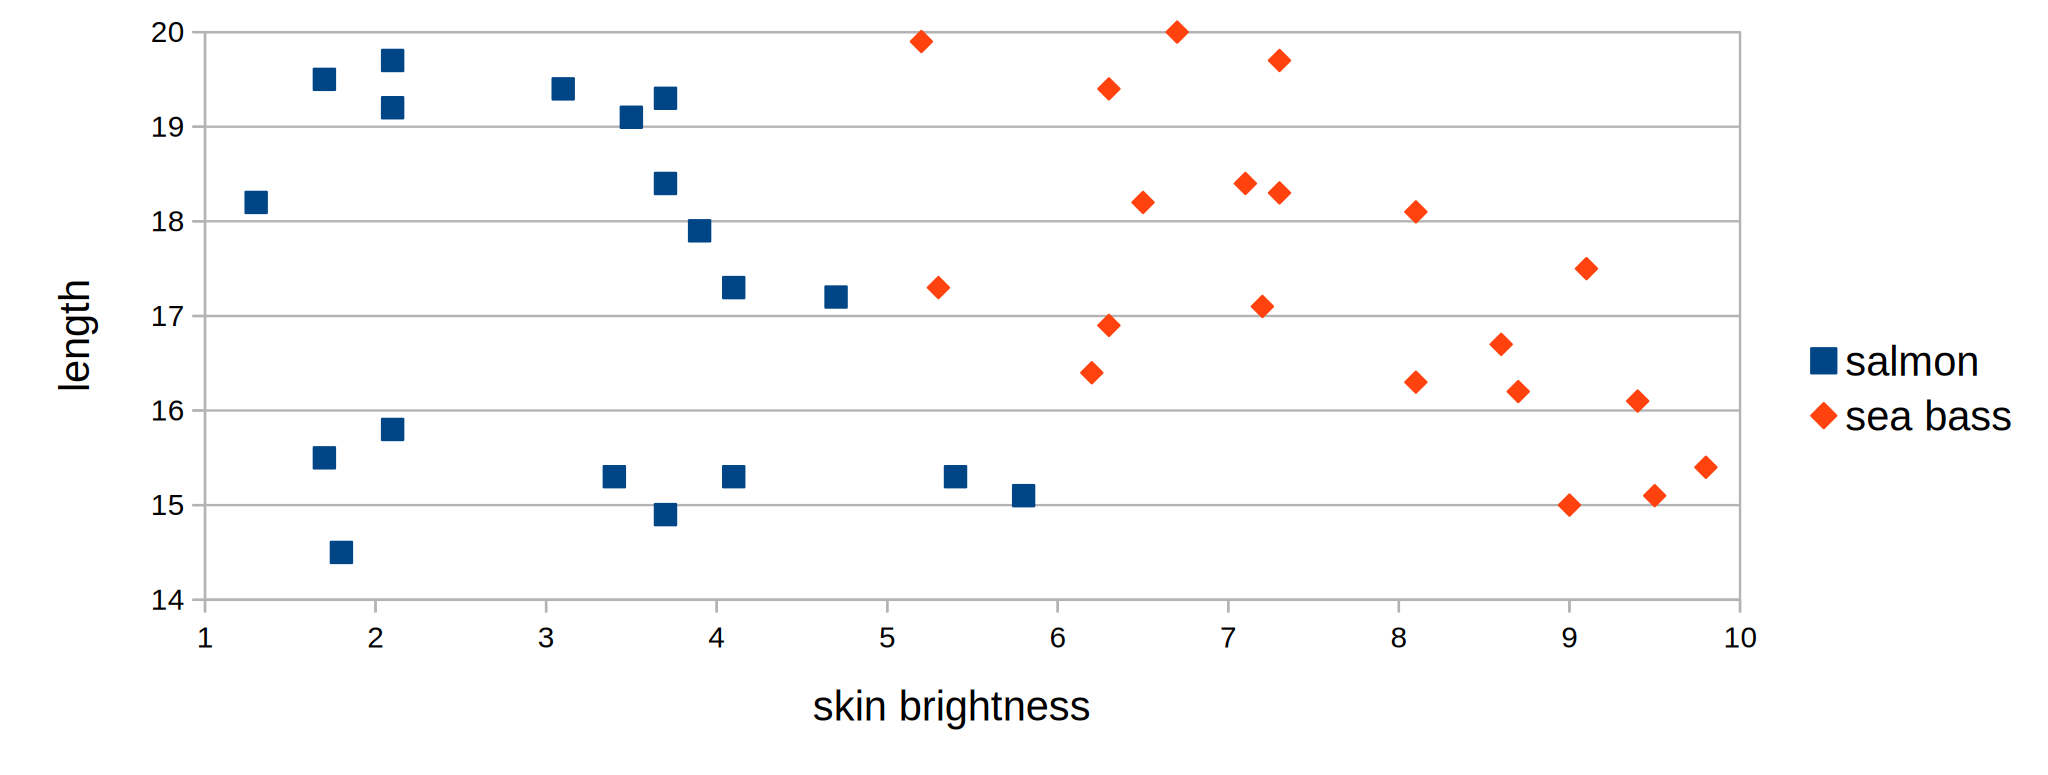
\includegraphics[width=.45\textwidth]{classification-fish.png}
\caption[Classification of fish]{Classification of fish species dependent on their length and skin brightness. The classification model should learn the decision boundary (pink) to successfully distinguish between the two fish species.}
\label{fig:fish-classification}
\end{figure}

For regression tasks the features within the input data are used to approximate other variables for the output. The output itself is unlike to classification tasks \textbf{numerical values} and not classes. \textit{Numerical values (input) are therefore used to approximate the values of one or more other numerical values (output)}. An example for this would be the approximated prediction of mileage of cars dependent on their motor power and weight. The regression model would learn a function that approximates the mileage (output) dependent on the input data, which consists of motor power and weight. This model then learned to generalize by the given data and can be used to predict the mileage of new cars it has not seen before dependent on the knowledge it gained before (given data).

\subsection{Unsupervised learning}
Unsupervised learning is used to find patterns in data without labels (unlabeled data). The input data does not have labeled output data. This means that nothing can be interpreted about the output data. So using unsupervised learning is often also called knowledge discovery. In real life most existent data is unlabeled or partially labeled. This leads to the conclusion that unsupervised learning finds often more usage. Unsupervised learning can be used to cluster data. This will group similar data input clusters. These clusters can then be further processed and put into class for example.

\subsection{\gls{connectionism}}
Connectionism tries to solve complex problems by modeling what we use to solve problems - our brain. Neurobiologically the brain consists on a low level of neurons that are connected. This can be modeled into a computer science abstraction. A neuron is 

\subsection{Deep learning}

\section{Reinforcement learning}
exploitation, exploration, thompson sampling, qlearning, sarsa

\section{Evolutionary computing}
TODO: EMMA
genetic algorithm, genetic programming, evolutionary programming

\section{Big Data in context}

\section{Current state of AI and further topics}
 - capsule networks
 - autoencoders
 - attention mechanisms
 - gans
 - dqn
 - neat
 - neuroevolution

\section{Further readings}
To get into the basics deeper and to learn more about some neural network architectures refer to \cite{Goodfellow-et-al-2016}. This book is available online and contains nearly everything you need to know about neural nets and deep learning.

\printglossaries
\printindex
\bibliography{ai-intro-article}

\end{document}
